
\section{Proposed methods}

\begin{frame}[plain]
   \sectionpage
\end{frame}

\frame{
   \frametitle{Outline}

   \textbf{Model-based approaches}
   \begin{itemize}
      \item \onlyh{2}{InfRed}{Improved lower bounds}
      \item Fix-and-optimize \emph{matheuristic}
   \end{itemize}

   \vspace*{24pt}

   \textbf{Meta-heuristic approaches}
   \begin{itemize}
      \item A biased random key genetic algorithm
      \item BRKGA with additional intensification components
   \end{itemize}
}

\subsection*{Model-based approaches}


\frame{
   \frametitle{Improved lower bounds}

   \textbf{Our experiments}
   \begin{itemize}
      \item MIP and objective weights of \citet{mankowska2014}
      \item Same model, \emph{smarter} building routines
      \item CPLEX 20.10 (Dec 2020)
%      \item 2 hours of processing
%      \item Single thread
%      \item Additional parameters to reduce memory consumption
%      \item MIP warm-start with one of our proposed meta-heuristics
   \end{itemize}

   \vspace{12pt}

   \textbf{Black-box tweaks}
   \begin{itemize}
      \item Additional parameters to reduce memory consumption
      \item MIP warm-start with one of our proposed meta-heuristics
   \end{itemize}

%   \begin{table}[H]
%      \centering
%      \scriptsize
%      \begin{tabular}{ll}
%         \toprule
%         Parameter & Tweaked value\\
%         \midrule
%         disable parallel processing &  \texttt{set threads 1}\\
%         turning on the reduced memory emphasis &  \texttt{set emphasis memory y}\\
%         set all cut generation to moderate &  \texttt{set mip cuts all 1}\\
%         disable clique cut generation &  \texttt{set mip cuts clique -1}\\
%         disable the probing on the root node &  \texttt{set mip strategy probe -1}\\
%         setting the branching direction to explore up first &  \texttt{set mip strategy branch 1}\\
%         setting the mip emphasis to improve the best bound &  \texttt{set emphasis mip 3}\\
%         fixing the random seed to 1 &  \texttt{set randomseed 1}\\
%         \bottomrule
%      \end{tabular}
%   \end{table}
}

\frame{
   \frametitle{Outline}

   \textbf{Model-based approaches}
   \begin{itemize}
      \item \onlyh{1}{InfRed}{Improved lower bounds}
      \item \onlyh{2}{InfRed}{Fix-and-optimize \emph{matheuristic}}
   \end{itemize}

   \vspace*{24pt}

   \textbf{Meta-heuristic approaches}
   \begin{itemize}
      \item A biased random key genetic algorithm
      \item BRKGA with additional intensification components
   \end{itemize}
}

\frame{
   \frametitle{Fix-and-Optimize \emph{matheuristic}}

   \textbf{Solving a MIP directly is very ineffective}
   \begin{itemize}
      \item Weak lower bounds \citep{gendreau2010}
      \item Feasibility issues
      \item Convergence issues
      \item Memory consumption
   \end{itemize}

   \vspace*{12pt}

   \textbf{The Fix-and-Optimize \emph{matheuristic}}
   \begin{itemize}
      \item Originally proposed by \citet{helber2010}
%      \item Applied by \citet{dorneles2014fix}
%      \item Also applied by \citet{chen2015}
      \item ``MIP-based local search''
   \end{itemize}
}

\frame{
   \frametitle{Fix-and-Optimize \emph{matheuristic}}

   \textbf{The Fix-and-Optimize \emph{matheuristic}}
   \begin{itemize}
      \item Still requires keeping the model in memory
      \item (Usually) requires a initial solution
   \end{itemize}

   \vspace*{8pt}

   % Define block styles
   \tikzstyle{decision} = [diamond, draw, fill=yellow!20,
   text width=4.5em, text badly centered, node distance=3cm, inner sep=0pt]
   \tikzstyle{block} = [rectangle, draw, fill=InfRed!20,
   text width=5em, text centered, rounded corners, minimum height=4em]
   \tikzstyle{line} = [draw, -latex']

   \begin{figure}[H]
      \centering
      \begin{tikzpicture}[node distance = 2.5cm, auto]
         \scriptsize
         \node [block] (init) {initial solution};
         \node [block, right of=init, node distance=2.8cm] (subproblem) {generate subproblem};
         \node [block, below of=subproblem] (optimize) {solver call};
         \node [decision, right of=optimize] (stop-criteria) {stop criteria achieved};
         \node [block, right of=stop-criteria, node distance=3cm] (finish) {finish};

         \path [line] (init) -- (subproblem);
         \path [line] (subproblem) -- (optimize);
         \path [line] (optimize) -- (stop-criteria);
         \path [line] (stop-criteria) |- node [near start] {no} (subproblem);
         \path [line] (stop-criteria) -- node [near start] {yes} (finish);
      \end{tikzpicture}
   \end{figure}

%   \begin{tikzpicture}[overlay]
%      \draw<2>[green,line width=2pt](-0.1, 3.6) rectangle (2.1, 5.18);
%   \end{tikzpicture}
}


%\frame{
%   \frametitle{Fix-and-Optimize \emph{matheuristic}}
%
%  \textbf{On the subproblem generation: decomposition}
%   \begin{itemize}
%      \item Removes variable fixing constraints
%      \item ``Variable unfixing''
%      \item Can remove as many constraints as desired
%   \end{itemize}
%
%   \vspace*{18pt}
%
%   \textbf{Choice of variables to unfix}
%   \begin{itemize}
%      \item Tractable subproblem
%      \item (Potentially) allowing solution improvement
%   \end{itemize}
%}
%
%\frame{
%   \frametitle{Fix-and-Optimize \emph{matheuristic}}
%
%   \textbf{The Fix-and-Optimize \emph{matheuristic}}
%   \begin{itemize}
%      \item Still requires keeping the model in memory
%      \item (Usually) requires a initial solution
%   \end{itemize}
%
%   \vspace*{8pt}
%
%   % Define block styles
%   \tikzstyle{decision} = [diamond, draw, fill=yellow!20,
%   text width=4.5em, text badly centered, node distance=3cm, inner sep=0pt]
%   \tikzstyle{block} = [rectangle, draw, fill=InfRed!20,
%   text width=5em, text centered, rounded corners, minimum height=4em]
%   \tikzstyle{line} = [draw, -latex']
%
%   \begin{figure}[H]
%      \centering
%      \begin{tikzpicture}[node distance = 2.5cm, auto]
%      \scriptsize
%      \node [block] (init) {initial solution};
%      \node [block, right of=init, node distance=2.8cm] (subproblem) {generate subproblem};
%      \node [block, below of=subproblem] (optimize) {solver call};
%      \node [decision, right of=optimize] (stop-criteria) {stop criteria achieved};
%      \node [block, right of=stop-criteria, node distance=3cm] (finish) {finish};
%
%      \path [line] (init) -- (subproblem);
%      \path [line] (subproblem) -- (optimize);
%      \path [line] (optimize) -- (stop-criteria);
%      \path [line] (stop-criteria) |- node [near start] {no} (subproblem);
%      \path [line] (stop-criteria) -- node [near start] {yes} (finish);
%      \end{tikzpicture}
%   \end{figure}
%
%   \begin{tikzpicture}[overlay]
%   \draw<1>[green,line width=2pt](2.7, 3.6) rectangle (4.91, 5.18);
%   \draw<2>[green,line width=2pt](2.7, 1.08) rectangle (4.9, 2.76);
%   \end{tikzpicture}
%}
%
%\frame{
%   \frametitle{Fix-and-Optimize \emph{matheuristic}}
%
%    \textbf{After decomposing}
%   \begin{itemize}
%      \item Calls the MIP optimizer
%      \item Usually a timeout is set (parameter ``step time limit'', or STL)
%      \item Generate new variable fixing constraints
%   \end{itemize}
%
%   \begin{tikzpicture}[overlay]
%      \draw<2>[InfRed,line width=2pt](-0.4, 0.35) rectangle (7.6, 0.98);
%      \node<2>[rectangle, fill=InfRed, anchor=south, text=white] at (3.8, -0.21) {Same solution, or a improved one};
%   \end{tikzpicture}
%}
%
%\frame{
%   \frametitle{Fix-and-Optimize \emph{matheuristic}}
%
%   \textbf{The Fix-and-Optimize \emph{matheuristic}}
%   \begin{itemize}
%      \item Still requires keeping the model in memory
%      \item (Usually) requires a initial solution
%   \end{itemize}
%
%   \vspace*{8pt}
%
%   % Define block styles
%   \tikzstyle{decision} = [diamond, draw, fill=yellow!20,
%   text width=4.5em, text badly centered, node distance=3cm, inner sep=0pt]
%   \tikzstyle{block} = [rectangle, draw, fill=InfRed!20,
%   text width=5em, text centered, rounded corners, minimum height=4em]
%   \tikzstyle{line} = [draw, -latex']
%
%   \begin{figure}[H]
%      \centering
%      \begin{tikzpicture}[node distance = 2.5cm, auto]
%      \scriptsize
%      \node [block] (init) {initial solution};
%      \node [block, right of=init, node distance=2.8cm] (subproblem) {generate subproblem};
%      \node [block, below of=subproblem] (optimize) {solver call};
%      \node [decision, right of=optimize] (stop-criteria) {stop criteria achieved};
%      \node [block, right of=stop-criteria, node distance=3cm] (finish) {finish};
%
%      \path [line] (init) -- (subproblem);
%      \path [line] (subproblem) -- (optimize);
%      \path [line] (optimize) -- (stop-criteria);
%      \path [line] (stop-criteria) |- node [near start] {no} (subproblem);
%      \path [line] (stop-criteria) -- node [near start] {yes} (finish);
%      \end{tikzpicture}
%   \end{figure}
%
%   \begin{tikzpicture}[overlay]
%      \draw<1>[green,line width=2pt](2.7, 1.08) rectangle (4.9, 2.76);
%      \draw<2>[green,line width=2pt](5.4, 0.55) rectangle (8.13, 3.15);
%   \end{tikzpicture}
%}
%
%\frame{
%   \frametitle{Fix-and-Optimize \emph{matheuristic}}
%
%   \textbf{Stopping criteria}
%   \begin{itemize}
%      \item Most common approach: iterations without improvement
%      \item Iters w/o improv: according to the size of the problem
%   \end{itemize}
%}
%
\frame{
   \frametitle{Fix-and-Optimize \emph{matheuristic}}

   \textbf{HHCRSP-specific F\&O:}
   \begin{itemize}
      \item Initial solution from \citeauthor{mankowska2014} constructive heuristic
      \item Keeps entire MIP in memory due to op. synchronizations
      \item Decomposition: optimizes \textit{two routes} at each iteration
   \end{itemize}

   \vspace*{12pt}

%   \textbf{Routes selection: selects caregivers $v_1 \neq v_2 \in \V$}
%   \begin{itemize}
%      \item At random (originally \emph{systematic decomposition})
%      \item Or guided, according patients' visit times
%   \end{itemize}
}

\frame{
   \frametitle{Outline}

   \textbf{Model-based approaches}
   \begin{itemize}
      \item Improved lower bounds
      \item \onlyh{1}{InfRed}{Fix-and-optimize \emph{matheuristic}}
   \end{itemize}

   \vspace*{24pt}

   \textbf{Meta-heuristic approaches}
   \begin{itemize}
      \item \onlyh{2}{InfRed}{A biased random key genetic algorithm}
      \item BRKGA with additional intensification components
   \end{itemize}
}

\subsection*{Meta-heuristic approaches}

\frame{
   \frametitle{Biased random key genetic alg.}

   \textbf{Base concept of RKGAs}
   \begin{itemize}
      \item Proposed by \citet{bean1994}
      \item Indirect representation
      \item Generic GA, needs a decoder
   \end{itemize}

   \begin{figure}[H]
      \centering
      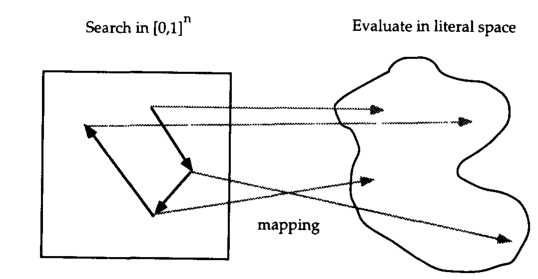
\includegraphics[width=0.6\textwidth]{fig/bean1994-rkga-decode.pdf}\\
      \footnotesize Source: \citet{bean1994}
   \end{figure}

%   \begin{tikzpicture}[overlay]
%      \draw<2,3>[green,line width=2pt](2.5, 1.26) rectangle (5.08, 4.5);
%      \node<3>[rectangle, fill=green, anchor=south, text=black] at (3.5, -0.21) {$v = \left(0.46 \quad 0.91 \quad 0.33 \quad 0.75 \quad 0.51\right)$};
%
%      \draw<5>[green,line width=2pt](6, 1.1) rectangle (8.76, 4.5);
%      \draw<4>[green,line width=2pt](5.1, 1.6) rectangle (6.1, 2.1);
%   \end{tikzpicture}
}


%\frame{
%   \frametitle{Biased random key genetic alg.}
%
%   \textbf{Elitism to improve convergence algorithm}
%   \begin{itemize}
%      \item So-called biased random key genetic algorithm \citep{gonccalves2011}
%      \item Split the population into elite and non-elite set
%      \item The elite set is kept from one generation to the next one
%%      \item As \emph{Monotonic} search
%      \item Improved crossover algorithm
%   \end{itemize}
%}
%
%\frame{
%   \frametitle{Biased random key genetic alg.}
%
%   \textbf{Basics elements of a BRKGA}
%   \begin{itemize}
%      \item \onlyh{2-4}{InfRed}{Initial population, mutants generation}
%      \item \onlyh{6-11}{InfRed}{Biased crossover, and the offspring}
%   \end{itemize}
%
%   \only<2-5>{
%      \vspace*{12pt}
%      \textbf{Initial population}
%      \begin{itemize}
%         \item \onlyh{3-4}{InfRed}{One can \emph{encode} a solution in random-keys space}
%         \item \onlyh{5}{InfRed}{Just sample a random number generator \texttt{PRNG(0,1)}}
%      \end{itemize}
%   }
%
%   \begin{tikzpicture}[overlay]
%      \node<4>[rectangle, fill=InfRed, anchor=south, text=white] at (3.5, -0.6) {Diversity loss, premature convergence!};
%   \end{tikzpicture}
%
%   \only<6-11>{
%      \begin{figure}[H]
%         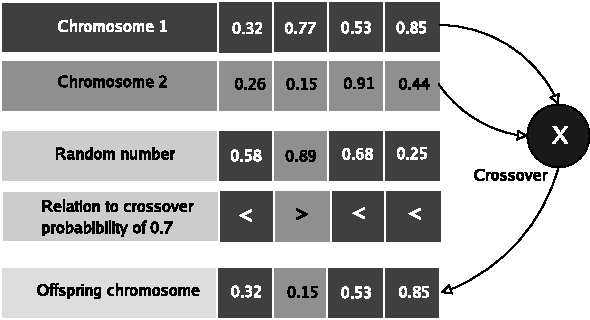
\includegraphics[width=0.7\textwidth]{fig/gonccalves2011-crossover.pdf}
%      \end{figure}
%   }
%
%   \begin{tikzpicture}[overlay]
%      \draw<7>[green,line width=2pt](1.55, 4.15) rectangle (7.35, 4.94);
%      \draw<8>[green,line width=2pt](1.55, 3.4) rectangle (7.35, 4.18);
%      \draw<9>[green,line width=2pt](4.4, 0.8) rectangle (5.13, 4.9);
%      \draw<10>[green,line width=2pt](5.13, 0.8) rectangle (5.85, 4.9);
%      \draw<11>[green,line width=2pt](1.55, 0.8) rectangle (7.35, 1.503);
%
%      \node<6-> at (5,0.3) {\footnotesize Source: \citet{gonccalves2011}};
%   \end{tikzpicture}
%}



\frame{
   \frametitle{Biased random key genetic alg.}

   \textbf{BRKGA}
   \begin{itemize}
      \item Proposed by \citet{gonccalves2011}
   \end{itemize}

   \vspace*{8pt}

   \begin{figure}[H]
      \centering
      \includegraphics[width=0.7\textwidth, page=2]{fig/brkga-framewk.pdf}
   \end{figure}
}

\frame{
   \frametitle{Biased random key genetic alg.}

   \textbf{For the home health care problem}
   \begin{itemize}
      \item BRKGA $\Rightarrow$ evolves the \emph{task insertion sequence}
      \item The proposed decoder \textbf{embeds} a greedy heuristic
      \item A \emph{best-insertion heuristic decoder} builds a routing solution from the TIS
   \end{itemize}

   \vspace*{12pt}

   \begin{figure}
      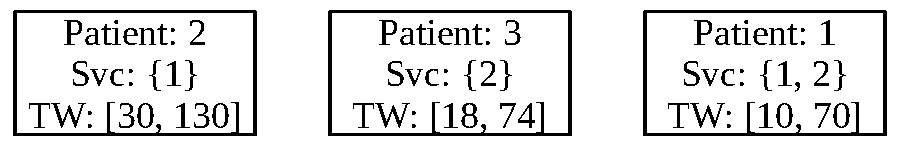
\includegraphics[width=0.6\textwidth]{fig/decoder-tis}
   \end{figure}

}

%\frame{
%   \frametitle{Biased random key genetic alg.}
%
%   \textbf{The task insertion sequence}
%   \begin{itemize}
%      \item Chromosome has many alleles than $|\C|$
%      \item Each allele represents a patient (and all their service requests)
%   \end{itemize}
%
%   \only<+> {
%      \vspace*{12pt}
%
%      \begin{figure}[H]
%         \centering
%         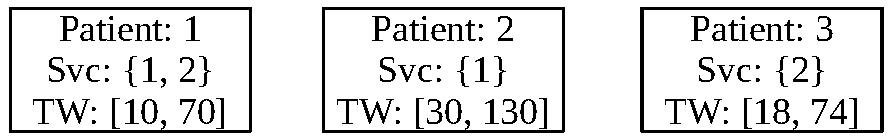
\includegraphics[width=0.7\textwidth]{fig/decoder-tasks.pdf}
%      \end{figure}
%
%      \begin{align*}
%         v = \left( 0.48 \quad 0.16 \quad 0.31 \right)
%      \end{align*}
%   }
%
%   \only<+> {
%      \vspace*{12pt}
%      \begin{figure}[H]
%         \centering
%         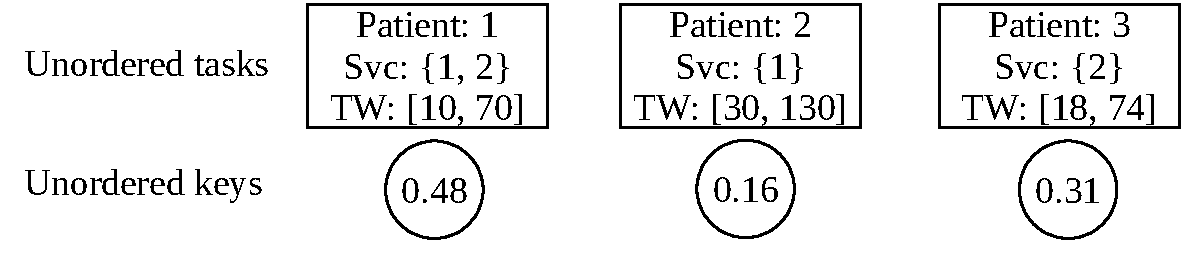
\includegraphics[width=0.8\textwidth]{fig/decoder-keys}
%      \end{figure}
%   }
%
%   \only<+> {
%      \vspace*{12pt}
%      \begin{figure}[H]
%         \centering
%         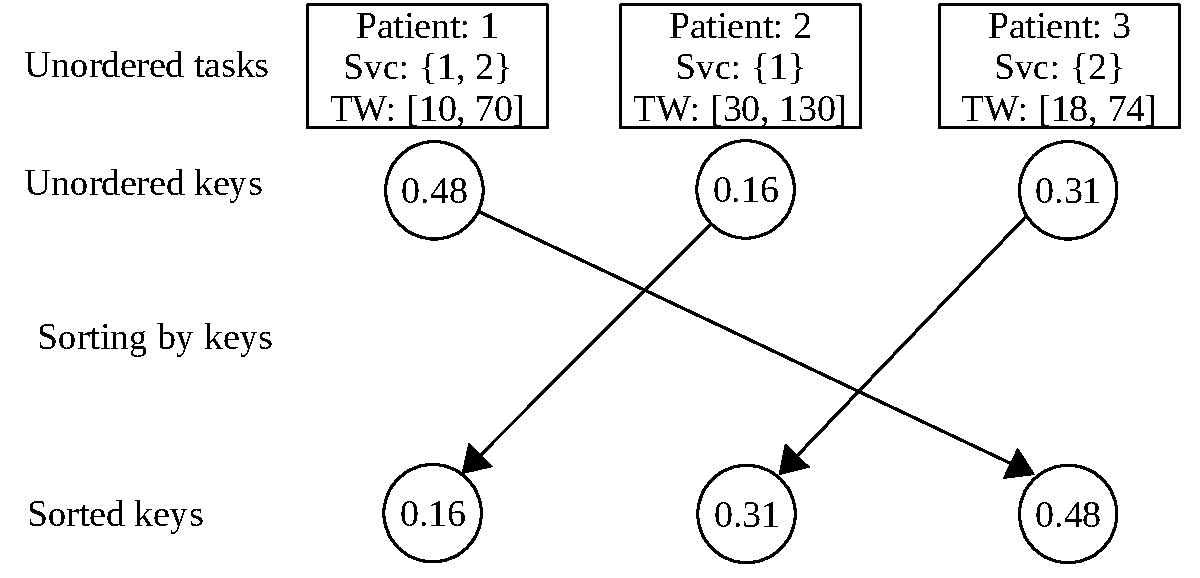
\includegraphics[width=0.8\textwidth]{fig/decoder-sort}
%      \end{figure}
%
%      \begin{tikzpicture}[overlay]
%         \draw[green,line width=2pt](1.2, 2.2) rectangle (3.2, 2.8);
%      \end{tikzpicture}
%   }
%
%   \only<+> {
%      \vspace*{12pt}
%      \begin{figure}[H]
%         \centering
%         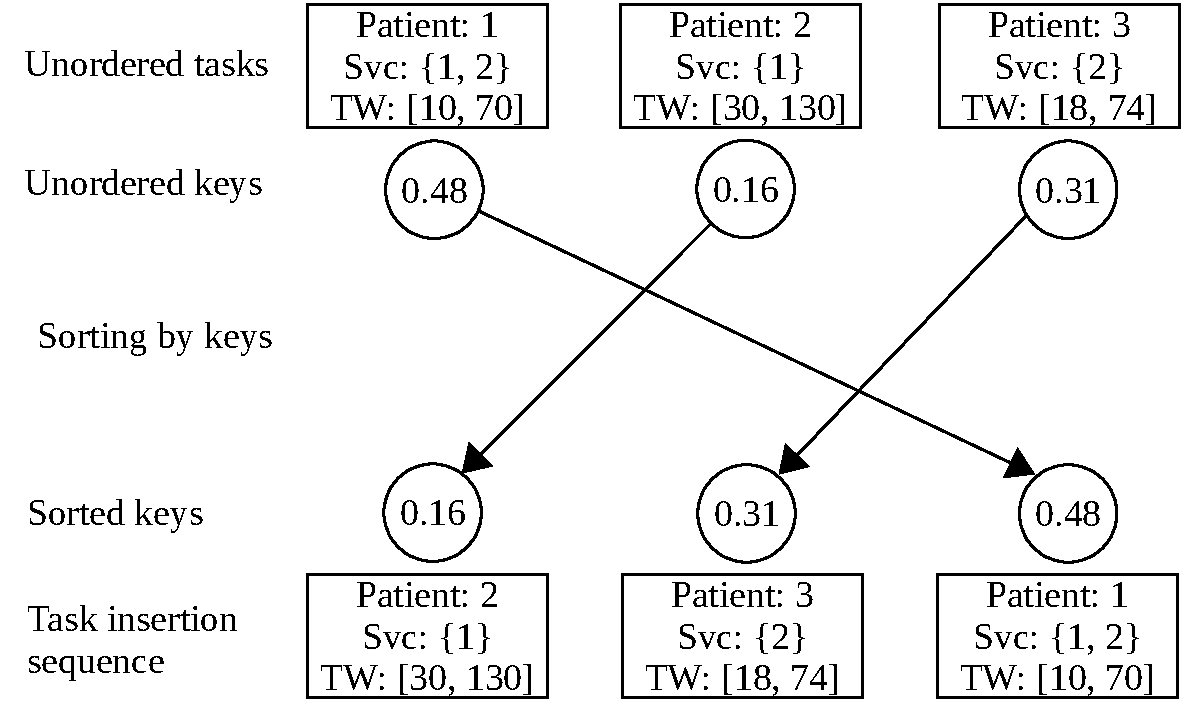
\includegraphics[width=0.8\textwidth]{fig/decoder}
%      \end{figure}
%   }
%
%%   \only<+>{
%%      \vspace*{12pt}
%%      \begin{figure}[H]
%%         \centering
%%         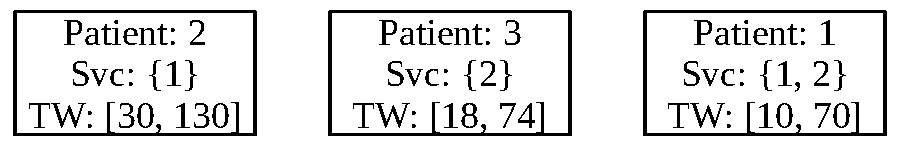
\includegraphics[width=0.8\textwidth]{fig/decoder-tis}
%%      \end{figure}
%%   }
%
%}

%\frame{
%   \frametitle{Biased random key genetic alg.}
%
%   \textbf{Best-insertion heuristic}
%   \begin{itemize}
%      \item Input: the task insertion sequence
%      \item All caregivers start at the depot
%      \item Greedily insert patient on caregiver routes
%      \item Finishes all routes at the depot
%   \end{itemize}
%
%   \vspace*{12pt}
%%
%%   \textbf{Guide the insertion according the objective function}
%%   \begin{itemize}
%%      \item Increment of travel times
%%      \item Increment of total tardiness
%%      \item Change of the maximum tardiness
%%      \item Terms combined according the weights $\lambda_1$, $\lambda_2$, and $\lambda_3$
%%   \end{itemize}
%
%
%
%}

%\frame{
%   \frametitle{Biased random key genetic alg.}
%
%   \textbf{Task insertion sequence}
%   \begin{figure}[H]
%      \centering
%      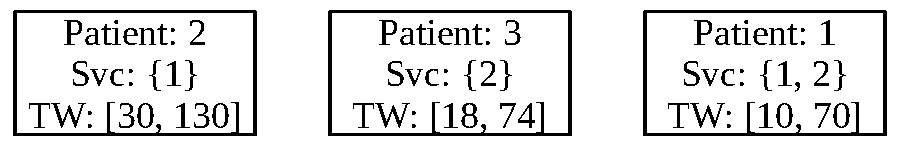
\includegraphics[width=0.6\textwidth]{fig/decoder-tis}
%   \end{figure}
%
%   \vspace*{8pt}
%
%
%   \textbf{Best-insertion heuristic}
%   \begin{figure}
%      \includegraphics<+>[width=0.95\textwidth,page=1]{fig/bi-heur}%
%      \includegraphics<+>[width=0.95\textwidth,page=2]{fig/bi-heur}%
%      \includegraphics<+>[width=0.95\textwidth,page=3]{fig/bi-heur}%
%      \includegraphics<+>[width=0.95\textwidth,page=4]{fig/bi-heur}%
%      \includegraphics<+>[width=0.95\textwidth,page=5]{fig/bi-heur}%
%      \includegraphics<+>[width=0.95\textwidth,page=6]{fig/bi-heur}%
%      \includegraphics<+>[width=0.95\textwidth,page=7]{fig/bi-heur}%
%      \includegraphics<+>[width=0.95\textwidth,page=8]{fig/bi-heur}%
%      \includegraphics<+>[width=0.95\textwidth,page=9]{fig/bi-heur}%
%      \includegraphics<+>[width=0.95\textwidth,page=10]{fig/bi-heur}%
%   \end{figure}
%
%%   \Todo{Incluir highlight no TIS durante a animação.}
%%   \Todo{Verificar se vale a pena inserir um terceiro \textit{caregiver} para demonstrar o comportamento do algoritmo.}
%}
%
%\frame{
%   \frametitle{Biased random key genetic alg.}
%
%   \textbf{Best-insertion heuristic}
%   \begin{itemize}
%      \item Consider caregiver qualification levels
%      \item Deals with double service patients
%%      \item Compute the shortest waiting times
%   \end{itemize}
%
%
%}

%\frame{
%   \frametitle{Biased random key genetic alg.}
%
%   \textbf{Best-insertion heuristic}
%   \begin{itemize}
%      \item It is not very expensive for small instances
%      \item $n = |\C|$, $m = |\V|$
%      \item Worst-case complexity of $O(nm^2)$
%      \item In practice, the cost is not so bad
%   \end{itemize}
%
%   \vspace*{8pt}
%
%   \begin{table}[H]
%      \footnotesize
%      \begin{tabular}{rrrr}
%         \toprule
%         $|\C|$ & $|\V|$ & Worst case & Empirical measure\\
%         \midrule
%         10 & 3 & 90 & 14\\
%         50 & 10 & 5,000 & 414 \\
%         100 & 20 & 40,000 & 2,571\\
%         200 & 30 & 180,000 & 12,892\\
%         300 & 40 & 480,000 & 26,996 \\ % 5.62\%  0.29 seconds 1 generation
%         \bottomrule
%      \end{tabular}
%   \end{table}
%}
%
%\frame{
%   \frametitle{Biased random key genetic alg.}
%
%   \textbf{Not always a bed of roses}
%   \begin{itemize}
%      \item The best-insertion heuristic is \textit{incomplete}
%      \item In some cases, it can not reach the optimal solution
%      \item Even though we known the optimal TIS
%   \end{itemize}
%
%   \vspace*{12pt}
%   \begin{figure}
%      \includegraphics<+>[width=0.4\textwidth, page=1]{fig/triangle.pdf}%
%      \includegraphics<+>[width=0.4\textwidth, page=2]{fig/triangle.pdf}%
%      \includegraphics<+>[width=0.4\textwidth, page=3]{fig/triangle.pdf}%
%      \only<+>{
%         \includegraphics[width=0.4\textwidth, page=4]{fig/triangle.pdf}\\
%         \footnotesize The final solution... \normalsize
%      }
%      \only<+>{
%         \includegraphics[width=0.4\textwidth, page=5]{fig/triangle.pdf}\\
%         \footnotesize ...but not the optimal one! \normalsize
%      }
%   \end{figure}
%}



\frame{
   \frametitle{Outline}

   \textbf{Model-based approaches}
   \begin{itemize}
      \item Improved lower bounds
      \item Fix-and-optimize \emph{matheuristic}
   \end{itemize}

   \vspace*{24pt}

   \textbf{Meta-heuristic approaches}
   \only<+> {
      \begin{itemize}
         \item \textcolor{InfRed}{A biased random key genetic algorithm}
         \item BRKGA with additional intensification components
      \end{itemize}
   }%
  \only<+> {
      \begin{itemize}
         \item A biased random key genetic algorithm
         \item \textcolor{InfRed}{BRKGA with additional intensification components}
      \end{itemize}
   }%
}

\frame{
   \frametitle{\footnotesize BRKGA with Intensification components}

   \textbf{Components of \citet{andrade2021}}
   \begin{enumerate}
      \item \onlyh{2}{InfRed}{Island model (also in \citet{toso2015})}
      \item Multi-parent mating
      \item Implicit path-relinking heuristic
   \end{enumerate}
}

\frame{
   \frametitle{\footnotesize BRKGA with Intensification components}

   \textbf{Island model}
   \begin{itemize}
      \item Island = a isolated population evolving by itself
      \item Standard BRKGA: single island
   \end{itemize}

   \vspace*{12pt}

   \textbf{Advantages}

   \begin{itemize}
      \item Immigration $\rightarrow$ Can find better solutions
      \item Helps keeping the diversity
      \item Shows better convergence than single-island approach
   \end{itemize}

   \vspace*{12pt}

   \textbf{Caveat: substantially more individuals to decode.}
}

\frame{
   \frametitle{\footnotesize BRKGA with Intensification components}

   \textbf{Components of \citet{andrade2021}}
   \begin{enumerate}
      \item \onlyh{1}{InfRed}{Island model (also in \citet{toso2015})}
      \item \onlyh{2}{InfRed}{Multi-parent mating}
      \item Implicit path-relinking heuristic
   \end{enumerate}
}

\frame{
   \frametitle{\footnotesize BRKGA with Intensification components}

   \textbf{Multi-parent mating}
%   \footnotesize
   \begin{itemize}
      \item Originally proposed by \citet{lucena2014-gd-mp}
      \item Objective: exploit good solution parts from several parents
      \item At least one elite parent
      \item At least one non-elite parent
      \item Implicit bias through weight functions of \citet{bresina1996-bias}
   \end{itemize}
%   \normalsize

%   \vspace*{12pt}
%   \textbf{Algorithmic view}
%   \footnotesize
%   \begin{enumerate}
%      \item Parent selection
%      \item Sort selected parents
%      \item Compute parent weight according to their \textit{rank}
%      \item Normalize the weights
%      \item Proceeds with a slightly modified mating algorithm of \citet{bean1994}
%   \end{enumerate}
%   \normalsize
}

%\frame{
%
%   \Todo{Acho que vale a pena adicionar um slide mostrando esse weight function operando no crossover}
%
%}

%\frame{
%   \frametitle{\footnotesize BRKGA with Intensification components}
%
%   \textbf{Path-relinking heuristic}
%%   \footnotesize
%   \begin{itemize}
%      \item Introduced by \citet{glover1997-pr}
%      \item Further discussed by \citet{resende2016-pr}
%      \item Acts as a \emph{directed} local-search algorithm
%   \end{itemize}
%%   \normalsize
%
%   \vspace*{12pt}
%
%   \textbf{Explore intermediate solutions}
%%   \footnotesize
%   \begin{itemize}
%      \item Common terminology: guide solution $g$, initial (or base) solution $b$
%      \item Incrementally replaces elements of $b$ with elements from $g$
%      \item Records the best solution found
%   \end{itemize}
%%   \normalsize
%
%}

\frame{
   \frametitle{\footnotesize BRKGA with Intensification components}

   \textbf{Components of \citet{andrade2021}}
   \begin{enumerate}
      \item Island model (also in \citet{toso2015})
      \item \onlyh{1}{InfRed}{Multi-parent mating}
      \item \onlyh{2}{InfRed}{Implicit path-relinking heuristic}
   \end{enumerate}
}

\frame{
   \frametitle{\footnotesize BRKGA with Intensification components}

   \textbf{Difficulties of implementing a PR}
   \begin{itemize}
      \item Efficient implementation can be challenging
      \item Variations of PR
      \item Hard to reuse: problem-dependent neighborhood
   \end{itemize}

   \vspace*{12pt}

   \textbf{Implicit path relinking come to the rescue!}
   \begin{itemize}
      \item Explores the solution space \textit{indirectly}
      \item Solutions encoded in random keys
   \end{itemize}
}

%\frame{
%   \frametitle{\footnotesize BRKGA with Intensification components}
%
%   \textbf{BRKGA with IPR}
%   \begin{itemize}
%%      \item Proposed by \citet{andrade2021}
%      \item Specialized IPR according to solution representation
%      \item In the case of the HHCRSP: permutation IPR
%   \end{itemize}
%
%   \vspace*{12pt}
%   \textbf{Permutation IPR}
%   \begin{itemize}
%      \item Given a guide individual, and a initial (or base) individual
%      \item Introduce the permutations of one individual into the other
%      \item Operates on the level of random keys
%   \end{itemize}
%
%}

%\frame{
%   \frametitle{\footnotesize BRKGA with Intensification components}
%
%   \textbf{Permutation IPR}
%
%   \begin{figure}
%      \centering
%      \includegraphics<1-3>[width=0.6\textwidth]{fig/ipr}
%      \includegraphics<4-6>[width=0.6\textwidth, page=2]{fig/ipr}
%   \end{figure}
%
%   \begin{tikzpicture}[overlay]
%%      \draw<+>[green,line width=2pt](2.8, 4.9) rectangle (8.8, 6);
%      \draw<2,3>[green,line width=2pt](3.605, 0.95) rectangle (4.65, 3.1
%      );
%      \draw<5,6>[green,line width=2pt](3.67, 0.95) rectangle (4.65, 3.1
%      );
%      \node<3>[rectangle, fill=green, anchor=south, text=black] at (0.8, 3.2) {$\operatorname{swap}(b_1, b_5)$};
%      \node<5,6>[rectangle, fill=green, anchor=south, text=black] at (4.15, 3.1) {\checkmark};
%      \draw<6>[green,line width=2pt](2.8, 4.9) rectangle (8.8, 6
%      );
%      \node<3>[rectangle, fill=green, anchor=south, text=black] at (0.8, 3.2) {$\operatorname{swap}(b_1, b_5)$};
%      \node<6>[rectangle, fill=green, anchor=south, text=black] at (3.5, -0.5) {Continues the decoding with the modified $b'$.};
%   \end{tikzpicture}
%}
%
%\frame{
%   \frametitle{\footnotesize BRKGA with Intensification components}
%
%   \textbf{BRKGA with IPR}
%   \begin{itemize}
%      \item The process repeats for each position of the chromosome
%      \item Each intermediate solution is evaluated by the decoder
%      \item In the worst case, calls the best-insertion heuristic $|\C|$ times
%      \item Worst case cost of $O(nm^2) \cdot n = O(n^2m^2)$
%      \item But the average cost, in practice, is cheaper
%   \end{itemize}
%
%   \begin{tikzpicture}[overlay]
%      \draw<2>[green,line width=2pt](-0.4, 1) rectangle (8, 1.6
%      );
%      \node<2>[rectangle, fill=green, anchor=south, text=black] at (3.5, -1.) {Recall $n = |\C|$ and $m = |\V|$.};
%%      \draw[] (0,0) grid (10,10);
%   \end{tikzpicture}
%
%}
%
%\frame{
%   \frametitle{\footnotesize BRKGA with Intensification components}
%
%   \textbf{BRKGA with IPR}
%   \begin{itemize}
%      \item Distance metrics
%      \item Typically tries a fixed number of pairs for IPR
%%      \item Best or random selection from the elite set
%      \item On multiple islands: tries IPR between elite individuals from distinct islands
%   \end{itemize}
%}

\frame{
   \frametitle{\footnotesize BRKGA with Intensification components}

%   \begin{algorithm}[H]
%      \caption{Outline of BRKGA-MP-IPR}
%      \tiny
%      $l \gets 0$\;
%      $\mathit{bestFitness} \gets \infty$\;
%      \For{$g \gets 1$ \textbf{to} $E^\mathit{tot}$} {
%         \tcp{BRKGA operations with multi-parent mating}
%         \For{$k' \gets 1$ \textbf{to} $k$} {
%            copy the elite set to the next population of $k'$\;
%            generate new mutants\;
%            fill the next population of $k'$ with offspring\;
%         }
%
%         \If{$g \mod E^\mathit{IPR}$}{
%            run the implicit path-relinking\;
%         }
%
%         \If{$g \mod E^\mathit{XE}$}{
%            run the immigration process\;
%         }
%
%         \eIf{a improved individual was found}{
%            update $\mathit{bestFitness}$\;
%            $l \gets 0$\;
%         }{
%            $l \gets l + 1$\;
%         }
%
%         \If{$l > E^\mathit{RST}$} {
%            replace all indviduals of the new population by mutants\;
%         }
%      }
%      \KwResult{Most fitted individual found.}
%   \end{algorithm}

   \textbf{BRKGA with Multi-Parent mating and IPR}
   \begin{enumerate}
      \item Initialize all islands with random individuals
      \item Mating and mutation
      \item Run implicit PR
      \item Exchange best individuals
   \end{enumerate}
}

